\label{sec:exercise_cm_gitlab_usage}

\section{Exercise CMGitLabUsage}

\subsection{Description of the M2Go Subgroup Structure}
The subgroup structure (figure \ref*{fig:screendump_subgroupStructure}) shows the Golang repository.
This repository consists out of three folder:
\begin{enumerate}
    \item BasicGoProgram/HelloWorld
    \item CarRental
    \item CarRentalCLI
\end{enumerate}
Further more there is the .gitignore file and the README.md file.

\begin{figure}[h]
    \centering
    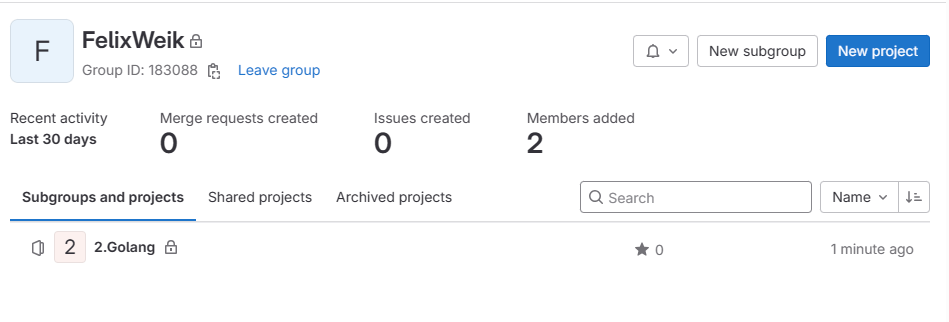
\includegraphics[width=0.8\textwidth]{figures/goLang/golang_personalSubgroupStructure.png}
    \caption{Screendump showing the subgroup structure}
    \label{fig:screendump_subgroupStructure}
\end{figure}

\subsection{Repository Cloning Steps}
To clone the repository, the following steps are required:
\begin{enumerate}
    \item Create a Personal Access Token (PAT) on GitLab by going to your profile settings and then to Access Tokens
    \item Save the PAT in a safe place
    \item Go to the repository and copy the HTTPS clone URL
    \item Open the WSL2 terminal and navigate to the folder where you want to clone the repository, in my case \texttt{/home/felix/WASA\_M2Go}
    \item Download the repository by running the following command in the terminal: \texttt{git clone <HTTPS clone URL>}
\end{enumerate}

\subsection{First Commit}
After changing the placeholder text in the README.md file, the first commit is done by using the graphical features Visual Studio Code offers.
The commit message (figure \ref*{fig:screendump_readmeCommitMessage}) is the following: \texttt{Update author and supervisor in README.md}.
After committing the changes, the changes are pushed to the remote repository, which then become visible on GitLab (figure \ref*{fig:screendump_readme}).

\begin{figure}[h]
    \centering
    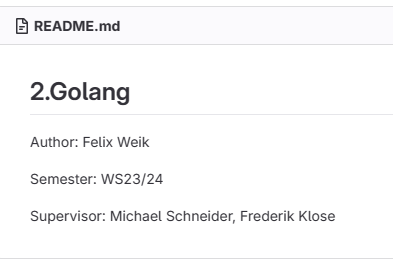
\includegraphics[width=0.5\textwidth]{figures/goLang/golang_screendumpReadme.png}
    \caption{Screendump showing the updated README.md file}
    \label{fig:screendump_readme}
\end{figure}

\begin{figure}[h]
    \centering
    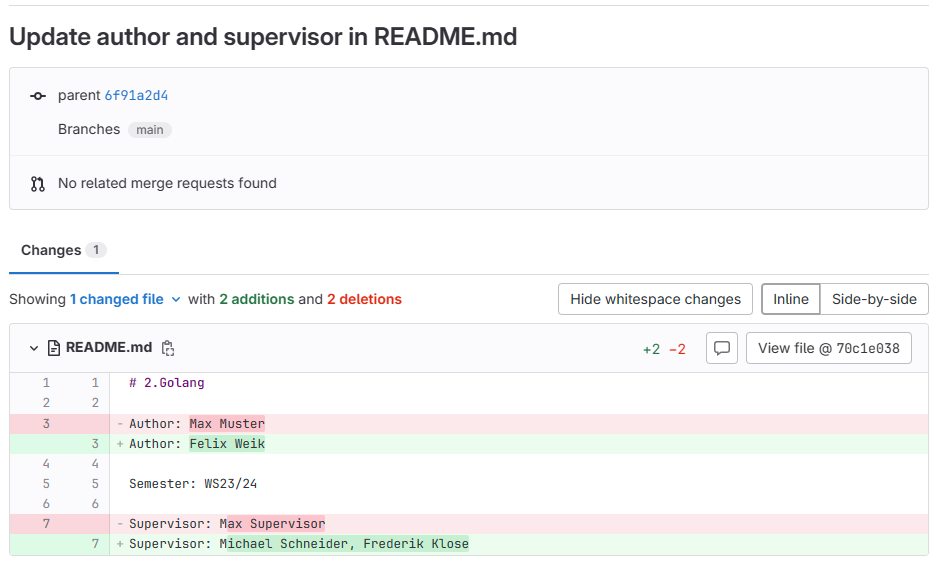
\includegraphics[width=0.8\textwidth]{figures/goLang/golang_screendumpReadmeCommit.png}
    \caption{Screendump showing commit message and the changed files}
    \label{fig:screendump_readmeCommitMessage}
\end{figure}